
\tikzset{dist1/.style={path picture= {
    \begin{scope}[x=1pt,y=10pt]
      \draw plot[domain=-6:6] (\x,{1/(1 + exp(-\x))-0.5});
    \end{scope}
    }
  }
}
\tikzset{dist2/.style={path picture= {
    \begin{scope}[x=1pt,y=10pt]
      \draw plot[domain=-6:6] (\x,{\x/10});
    \end{scope}
    }
  }
}
\tikzstyle{input}=[draw,fill=red!10,circle,minimum size=15pt,inner sep=0pt]
\tikzstyle{hidden}=[draw,fill=green!20,circle,minimum size=15pt,inner sep=0pt]
\tikzstyle{output}=[draw,fill=blue!20,circle,minimum size=15pt,inner sep=0pt]
\tikzstyle{bias}=[draw=none,circle,minimum size=15pt,inner sep=0pt]


\tikzstyle{stateTransition}=[->,line width=0.25pt,draw=black!50]


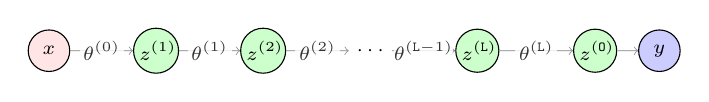
\begin{tikzpicture}[scale=1.36]\scriptsize
    \node (x)[input]   at (0, 1.5) {$\bm{x}$};
    \node (z1)[hidden] at (1, 1.5) {$\,\bm{z}^{(1)}$};
    \node (z2)[hidden] at (2, 1.5) {$\,\bm{z}^{(2)}$};
    \node (zi) at (3, 1.5) {$\cdots$};
    \node (zL)[hidden] at (4, 1.5) {$\,\bm{z}^{(\mathtt{L})}$};
    \node (zO)[hidden] at (5.1,1.5) {$\,\bm{z}^{(\mathtt{O})}$};
        %\node (zO)[hidden,fill=cyan!20] at (5.1,1.5) {$\,\bm{z}^{\!(\mathtt{O})}$};

    \node (y)[output] at (5.7,1.5) {$\bm{y}$};
   
   
    \draw[stateTransition,opacity=1] (x) -- (z1) node [midway, rotate=0,fill=white,opacity=0.8] {\scriptsize$\!\bm{\theta}^{(0)}\!$};
    \draw[stateTransition,opacity=1] (z1) -- (z2) node [midway, rotate=0,fill=white,opacity=0.8] {\scriptsize$\!\bm{\theta}^{(1)}\!$};
     \draw[stateTransition,opacity=1] (z2) -- (zi) node [midway, rotate=0,fill=white,opacity=0.8] {\scriptsize$\!\bm{\theta}^{(2)}\!$};
     \draw[stateTransition,opacity=1] (zi) -- (zL) node [midway, rotate=0,fill=white,opacity=0.8] {\scriptsize$\!\!\bm{\theta}^{(\mathtt{L}\text{-}1)}\!\!$};
    \draw[stateTransition,opacity=1] (zL) -- (zO) node [midway, rotate=0,fill=white,opacity=0.8] {\scriptsize$\!\bm{\theta}^{(\mathtt{L})}\!$};
     \draw[stateTransition,opacity=1] (zO) -- (y);
\end{tikzpicture}
